\documentclass[twocolumn, english]{revtex4-2}
\usepackage{amsmath}
\usepackage{braket}
\usepackage{titlesec}
\usepackage{graphicx}
\graphicspath{ {./images/} }
\numberwithin{equation}{section}
\begin{document}

\title{Quantum K-means Clustering}
\author{Rupak Chattarjee}
\email{Rupak.Chattarjee@stevens.edu}
\author{Abhijat Sarma}
\email{absarma@ctemc.org}
\affiliation{Center for Quantum Science and Engineering\\
Department of Physics, Stevens Institute of Technology, Castle Point on the Hudson, Hoboken, NJ 07030}
\begin{abstract}
Various machine learning classification algorithms, namely Support Vector Machines (SVMs), and K-means clustering, perform well on classifying wide ranges of datasets due to their versatility. However, as one increases the amount of data points and features, the computation time for training and using these statistical models grows intractably. Here, we attempt to use quantum analogues to these algorithms to lower the computational complexity of these models. We analyze a previously developed quantum SVM, as well as a quantum \textit{K}-means clustering algorithm we developed, on trinary classification of a real dataset. We find that our quantum clustering algorithm can classify linear boundaries much faster than and at least as accurately as SVMs and classical clustering algorithms.
\end{abstract}
\maketitle

\section{Introduction}
Machine learning offers solutions to several classes of problems unreachable through conventional computing means. For example, solutions to classification problems and regression of large datasets based on machine learning techniques are in general much more powerful than previously available solutions. Here, we focus specifically on classification algorithms. So-called Support Vector Machines (SVMs) are one such algorithm, suited to binary classification problems with broad applications to many different kinds of datasets. It is a family of supervised learning algorithms, meaning that it must first be “trained” on a dataset with known classifications, based on finding linear boundaries to datasets which are not necessarily linearly separable. Their power stems from their reliance on kernels, a typically nonlinear distance function, interpreted as an inner product in a higher dimensional space. SVMs use kernels to implicitly map input vectors to these higher, not necessarily finite dimensional, so-called "feature spaces", in which a separating hyperplane can be found. This ability to find linear separation boundaries in feature space, regardless of the shape of the decision boundary in input space, allows SVMs to be very versatile in their application. Additionally, kernel functions can be calculated without explicitly mapping each input vector to its representation in feature space, a technique known as the "kernel trick", saving lots of computational time. Despite their power, an insurmountable issue arises with regards to these machines: namely, that computation time of kernels tends to scale exponentially with the size and dimension of the datasets used. This problem can be circumvented using quantum computing methods. Two approaches to this problem exist: namely, direct implementation of the Support Vector Machine on a variational quantum circuit which is then optimized, as detailed in [2, 3], or direct computation of kernels on a quantum circuit which is then used to classically compute the Support Vector Machine. Here, the latter approach is investigate. We implement and characterize the algorithm introduced in [1], and compare it to a Radial Basis Function (RBF) classical kernel. 

Another algorithm we investigate is the \textit{K}-means clustering algorithm. It is an unsupervised clustering algorithm in which the dataset is arranged into \textit{K} clusters of similar datapoints. The algorithm relies on a distance measure, here taken to be Euclidean square distance. This distance can be calculated more efficiently on a quantum computer, as we will show, in order to speed up the algorithm as a whole. We compare our quantum K-means clustering algorithm to a classical one, as well as a quantum and classical multiclass extension of the SVM in solving trinary classification problems on a real dataset. We begin the paper with introductions of classical SVMs and \textit{K}-means clustering algorithms. Skip sections 2 and 4 if you are already familiar with these concepts.

\section{Support Vector Machine}

In machine learning theory, it is often mathematically convenient to consider the data as encoded in a vector. Therefore, each data point with \textit{P} different variables (features), can be encoded as a \textit{P}-dimensional feature vector. The total dataset is therefore a set of vectors in \textit{P}-dimensional space, known as input space. The support vector machine algorithm attempts to find a separating hyperplane - informally, an $\textit{M}-1$ dimensional generalization of a line - in \textit{M}-dimensional \textit{feature space} (a higher dimensional vector space of nonlinearly transformed feature vectors) from which all of the data points in one class will lie on one side of the hyperplane, and all of the data points in the other class will lie on the other. Let us consider a dataset consisting of \textit{N} different feature vectors $\textbf{X}^{i} = (\textit{X}^{i}_{1}, \textit{X}^{i}_{2}, …, \textit{X}^{i}_{P})$. The problem boils down to the convex optimization problem of finding the factors $\alpha^{i}$ such that \begin{equation}f(\textbf{X})=\sum_{i=1}^{N}\alpha^{i}y^{i}K(\textbf{X}^{i}, \textbf{X})+b\end{equation} is a decision function acting on a datapoint $\textbf{X}$ whose sign correctly classifies it - namely, positive values of f(\textbf{X}) correspond to one classification for \textbf{X}, and negative values correspond to the other. See [8] for more information. $\textit{K}(\textbf{X}, \textbf{X}^{i})$ is a positive-definite \textit{kernel} function, equal to an inner product in some high dimensional vector space. \begin{equation}\textit{K}(\textbf{X}, \textbf{X}^{i})=\sum_{j}^{\infty}\varphi_{j}(\textbf{X}^{i})\varphi(\textbf{X}).\end{equation} Here, $\varphi$ is some non-linear transformation into higher dimensional vector space. The power of the SVM stems from the fact that the kernel function can be calculated without explicitly calculating $\varphi$. Different kernels give rise to different decision boundaries, but many kernels are classically intractable. However, some can be more efficiently calculated on a quantum computer, as will be explored in the next section.

\section{The Quantum Support Vector Machine}

In this section, we switch to the notation $\vec{x}$ instead of $\textbf{X}^{i}$ to denote our feature vectors to avoid indexing confusion. To achieve calculation of a classically intractable kernel, we must encode the feature vectors $\vec{x}$ into quantum states that can be manipulated to compute our desired kernel. Here, we explore one such algorithm. Note that the algorithm presented here was developed by Havlicek et al. in [1]. We define the unitary gate \begin{equation}\textbf{U}_{\Phi(\vec{x})}=\exp(i\sum_{S\subseteq[n]}\phi_{S}(\vec{x})\prod_{i\in S}Z_{i}),\end{equation} as well as the n-qubit gate \begin{equation}\textbf{M}_{\Phi(\vec{x})}=\textbf{U}_{\Phi(\vec{x})}\textbf{H}^{\otimes n}\textbf{U}_{\Phi(\vec{x})}\textbf{H}^{\otimes n}\end{equation} where \textbf{H} is the usual Hadamard gate. Here we take $n=2$. The data is encoded through the coefficients $\phi_{S}(\vec{x})$, such that \begin{equation}\phi_{1}(\vec{x})=x^{i}, \phi_{1, 2}(\vec{x})=(\pi-x^{1})(\pi-x^{2})\end{equation} We define our kernel as follows \begin{equation}K(\vec{x}, \vec{z})=|\braket{\Phi(\vec{x})|\Phi(\vec{z})}|^2 = |\braket{0^n|\textbf{M}^{\dag}_{\Phi(\vec{x})}\textbf{M}_{\Phi(\vec{z})}|0^n}|^2. \end{equation} This kernel is thought to be classically intractable. However, it can be easily calculated by applying the gate $\textbf{M}_{\Phi(\vec{x})}$ followed by the gate $\textbf{M}^{\dag}_{\Phi(\vec{z})}$ to an initial state $\ket{0}^{n}$and experimentally calculating the frequency of getting the zero strings $0^n$ as a result from the circuit. 

\section{\textit{K}-means Clustering}

\textit{K}-means clustering is an unsupervised learning algorithm which considers the problem of partitioning \textit{N} feature vectors into \textit{K} \textit{subsets}, or \textit{clusters}. The algorithm seeks to find the \textit{K} clusters which minimize the dissimilarity between each cluster's members. Consider a dissimilarity metric between two features $\textit{D}(\textbf{X}^{i}, \textbf{X}^{j})$, which has the characteristic property that it increases in value as the features $\textbf{X}^{i}, \textbf{X}^{j}$ become more dissimilar. The measure used does not necessarily have to be a metric. Let \textit{$d_{k}(X_{k}^{(i)}, X_{k}^{(j)})$} be a dissimilarity measure between the \textit{$k^{th}$} features of two observations $\textbf{X}^{i}$ and $\textbf{X}^{j}$. The canonical dissimilarity measure for clustering is then \begin{equation}\textit{D}(\textbf{X}^{i}, \textbf{X}^{j})=\sum_{p=1}^\textit{P} \textit{w}_{p} \cdot \textit{$d_{p}(X_{p}^{(i)}, X_{p}^{(j)})$}, \sum_{p=1}^\textit{P} \textit{w}_{p} = 1\end{equation} where $\textit{w}_{p}$ are weights for the different features. The standard choice for \textit{$d_{p}(X_{p}^{(i)}, X_{p}^{(j)})$} is the squared distance  \begin{equation}d_{p}(X_{p}^{(i)}, X_{p}^{(j)}) = (X_{p}^{(i)} - X_{p}^{(j)})^2.\end{equation} For continuous, real feature variables, the canonical dissimilarity measure with $\textit{w}_{k} = 1$ becomes the squared Euclidean distance, \begin{equation}\textit{D}(\textbf{X}^{i}, \textbf{X}^{j})=d_{p}(X_{p}^{(i)}, X_{p}^{(j)})=|\textbf{X}^{i}-\textbf{X}^{j}|^2.\end{equation} The \textit{K}-means clustering algorithm is initialized with some \textit{K} clusters \textit{$C_{1}, C_{2}, ..., C_{K}$} Each observation $\textbf{X}^{i}$ belongs to one and only one cluster. The goal is to create clusters of observations that are the least dissimilar. The canonical intra-cluster measurement of this dissimilarity is \begin{equation}E(\textit{C}_{k}) = \frac{1}{|C_{k}|}\sum_{i, j \in{C_{k}}}\sum_{p=1}^{\textit{P}}(X_{p}^{(i)} - X_{p}^{(j)})^2\end{equation} Defining \textit{$m_{kp}$} as the \textit{mean} of feature \textit{p} in cluster \textit{k}, \begin{equation}\textit{$m_{kp}$}=\frac{1}{|C_{k}|}\sum_{i\in{C_{k}}}X_{p}^{(i)},\end{equation} one can express the \textit{energy} term (5.4) as variance from the mean, \begin{equation}E(\textit{C}_{k}) = 2\sum_{i\in{C_{k}}}\sum_{p=1}^{\textit{P}}(X_{p}^{(i)}-m_{kp})^2.\end{equation} In order to fulfill the least dissimilar criteria, one must minimize a cost function equal to the sum of each cluster's energy,\begin{equation}min_{\{C_{1}, C_{2}, ..., C_{K}\}}\left\{\sum_{k=1}^{K}E(C_{k})\right\}.\end{equation} This minimization is most commonly achieved with \textit{Lloyd's Algorithm}, as follows: \newline
\underline{\textbf{Lloyd's Algorithm}}
\begin{enumerate}
\item Randomly assign a cluster assignment \{1, 2, ..., \textit{K}\} to each of the observations $\textbf{X}^{i}$.
\item For each cluster $C_{k}$, calculate the \textit{vector of feature means} ($m_{k1}, m_{k2}, ..., m_{kP}$) called the cluster's \textit{centroid}
\item Assign each observation $\textbf{X}^{i}$ to the cluster $C_{k}$ with the closest centroid according to the Euclidean metric (5.3)
\item Iterate between 2 and 3 until the assignments to clusters do not change.
\end{enumerate}
The required number of iterations can be lowered by cleverly choosing the initial cluster assignments, such as by the \textit{K}-means++ algorithm, but that will not be explored in this paper. Sampling and estimating Euclidean distances between post-processed vectors on a classical computer is known to be exponentially hard. For big data sets, the algorithm becomes slow as convergence relies on repeated calculations of this distance measure. In the next section, we propose and implement a quantum algorithm for calculating the Euclidean distance, which can be shown to be exponentially faster than the classical counterpart [4]. Note that although we use Euclidean distance in our clustering algorithm, one could use any distance measure. The Euclidean distance is desirable for our purposes because it utilizes linear decision boundaries between clusters. For non-linear boundaries, one could use a corresponding distance measure. 
\section{Quantum K-means Clustering}
To develop our quantum algorithm for estimation of Euclidean distance, we first must introduce the \textit{swap test}. Consider a state \begin{equation}\ket{0}\otimes\ket{\psi}\otimes\ket{\varphi},\end{equation} consisting of an ancillary qubit and two equal-qubit states which we wish to find the overlap of. Perform a Hadamard transformation \textbf{H} on the ancillary followed by a \textbf{FREDKIN} gate (also known as a \textit{controlled swap}) on this state, \begin{equation}\begin{gathered}
\textbf{FREDKIN}(\textbf{H}\otimes\textbf{I}\otimes\textbf{I})\ket{0}\otimes\ket{\psi}\otimes\ket{\varphi}\\
=(\ket{0}\bra{0}\otimes\textbf{I}\otimes\textbf{I}+\ket{1}\braket{1|\textbf{SWAP}})\frac{1}{\sqrt{2}}[\ket{0}\otimes\ket{\psi}\otimes\ket{\varphi}\\+\ket{1}\otimes\ket{\psi}\otimes\ket{\varphi}]\\
=\frac{1}{\sqrt{2}}[\ket{0}\otimes\ket{\psi}\otimes\ket{\varphi}+\ket{1}\otimes\ket{\varphi}\otimes\ket{\psi}]\end{gathered}\end{equation}
Applying the Hadamard transformation once more to the ancillary qubit gives
\begin{equation}\begin{gathered}
\ket{\Psi}=(\textbf{H}\otimes\textbf{I}\otimes\textbf{I})\frac{1}{\sqrt{2}}[\ket{0}\otimes\ket{\psi}\otimes\ket{\varphi}\\+\ket{1}\otimes\ket{\varphi}\otimes\ket{\psi}]\\
=\frac{1}{2}[(\ket{0}+\ket{1})\otimes\ket{\psi}\otimes\ket{\varphi}\\+(\ket{0}-\ket{1})\otimes\ket{\varphi}\ket{\psi})]\\
=\frac{1}{2}\ket{0}\otimes[\ket{\psi}\otimes\ket{\varphi}+\ket{\varphi}\otimes\ket{\psi}]\\+\frac{1}{2}\ket{1}\otimes[\ket{\psi}\otimes\ket{\varphi}-\ket{\varphi}\otimes\ket{\psi}]
\end{gathered}\end{equation}
Finally, measure the state of the ancillary qubit. The probability of measuring $\ket{0}$ is given by 
\begin{equation}\begin{gathered}
\braket{\Psi|(\ket{0}\bra{0}\otimes\textbf{I}\otimes\textbf{I})|\Psi}\\=\frac{1}{4}\{\bra{\psi}\otimes\bra{\varphi}+\bra{\varphi}\otimes\bra{\psi}\}[\ket{\psi}\otimes\ket{\varphi}+\ket{\varphi}\otimes\ket{\psi}]\\
=\frac{1}{2}+\frac{1}{4}[(\bra{\psi}\otimes\bra{\varphi})(\ket{\varphi}\otimes\ket{\psi})\\+(\bra{\varphi}\otimes\bra{\psi})(\ket{\psi}\otimes\ket{\varphi})]\\
=\frac{1}{2}+\frac{1}{4}[\braket{\psi|\varphi}\braket{\varphi|\psi}+\braket{\varphi|\psi}\braket{\psi|\varphi}]
\end{gathered}\end{equation}
Therefore, as first shown in [5],
\begin{equation}
P[\ket{0}] = \braket{\Psi|(\ket{0}\bra{0}\otimes\textbf{I}\otimes\textbf{I})|\Psi} = \frac{1}{2}+\frac{1}{2}|\braket{\psi|\varphi}|^2
\end{equation}
The swap test therefore allows us to experimentally determine the overlap between two states $\ket{\psi}$ and $\ket{\varphi}$. This will be integral in calculating the Euclidean distance. In order to calculate Euclidean distance, we must first encode our feature vectors into Hilbert Space. We do this by encoding the vectors into quantum states using the base-2 \textit{bit string configuration} introduced in [6]. Recall that $\ket{p}=\ket{p_{n-1}p_{n-2}...p_{1}p_{0}}, p=2^{0}p_{0}+2^{1}p_{1}+...2^{n-1}p_{n-1}, P=2^{n}$. Note that if the dimension of the feature vector $\textbf{X}^{i}$ is not a power of two, one must pad it with zeroes in order to make it such. 
\begin{equation}
\ket{\textbf{X}^i} = \frac{1}{|\textbf{X}^i|}\sum_{p=1}^{P} X_{p}^{(i)}\ket{p}
\end{equation}
Realize that the overlap between two of these states recovers the usual vector dot product, namely
\begin{equation}
\braket{\textbf{X}^{i}|\textbf{X}^{j}}=\frac{1}{|\textbf{X}^{i}||\textbf{X}^{j}|}\sum_{p=1}^{P}X_{p}^{(i)}X_{p}^{(j)}=\frac{1}{|\textbf{X}^{i}||\textbf{X}^{j}|}\textbf{X}^{i}\cdot\textbf{X}^{j}
\end{equation}

\begin{figure*}
\scalebox{0.3}{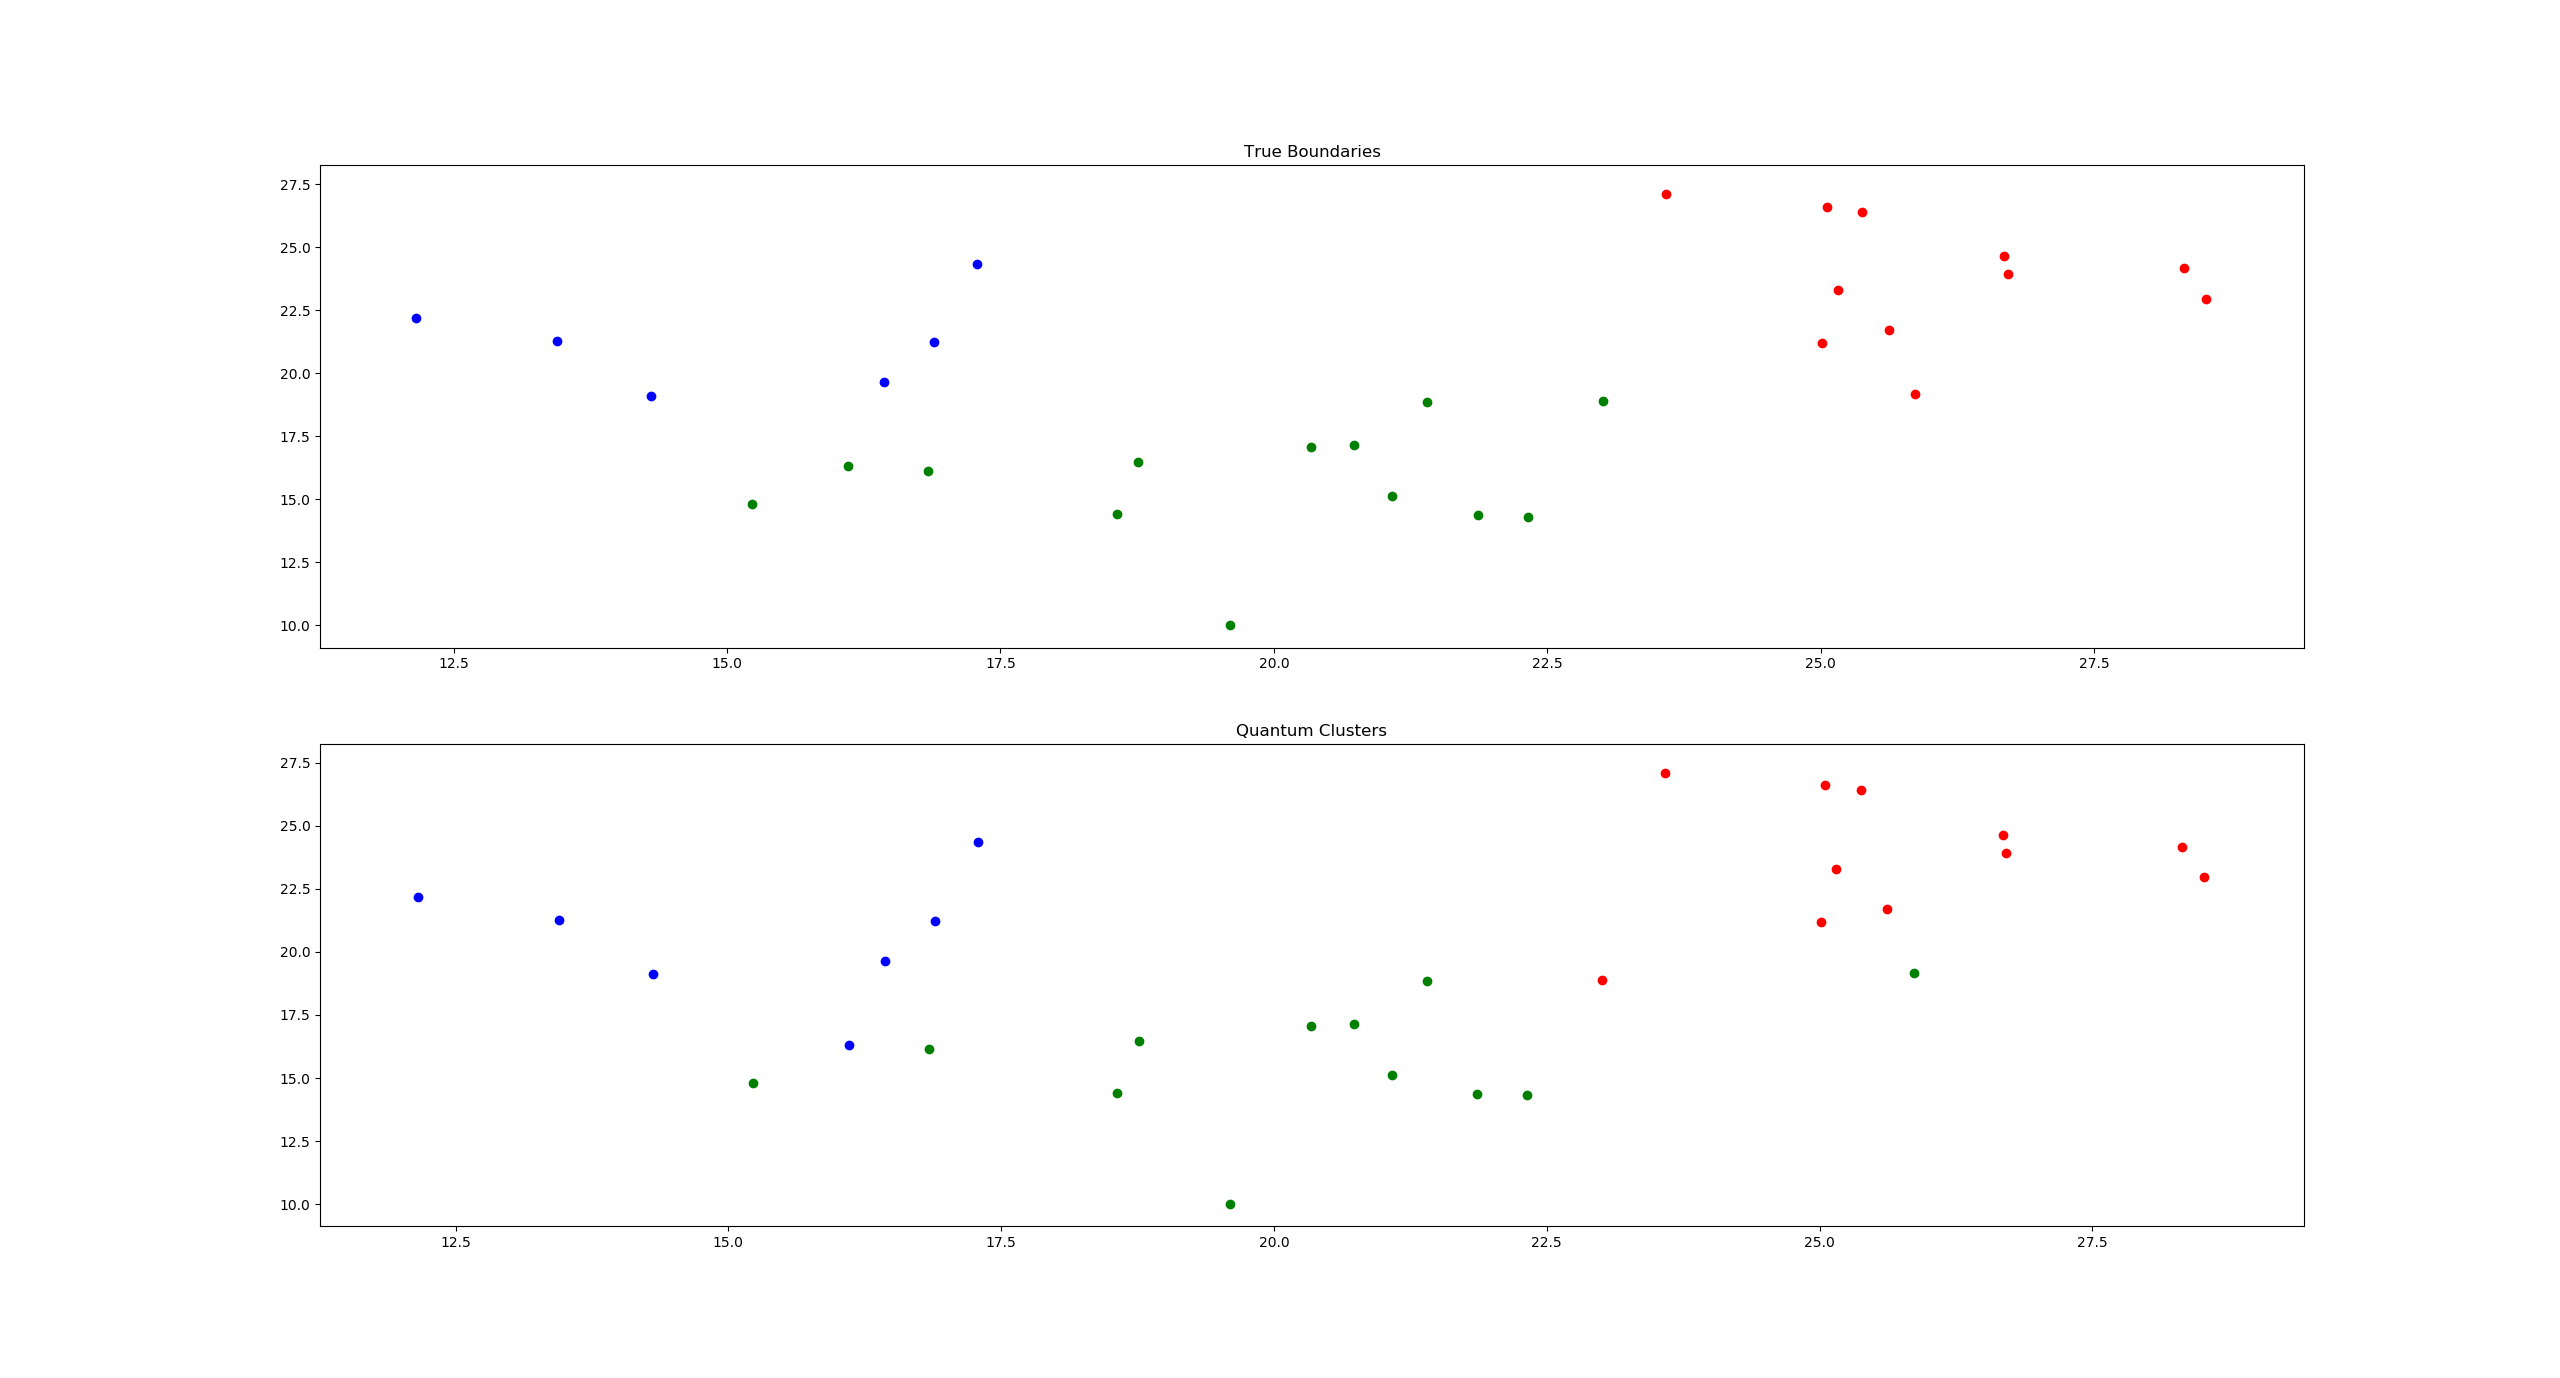
\includegraphics{Figure_1}}
\caption{True and Predicted Classifications by Quantum K-means algorithm}
\end{figure*}

Next, we construct the following states
\begin{equation}\begin{gathered}
\ket{\psi}=\frac{1}{2}[\ket{0}\otimes\ket{\textbf{X}^{i}}+\ket{1}\otimes\ket{\textbf{X}^{j}}]\\
\ket{\varphi}=\frac{1}{Z}[|\textbf{X}^{i}|\ket{0} - |\textbf{X}^{j}|\ket{1}]
\end{gathered}\end{equation}
where $Z = |\textbf{X}^{i}|^2+|\textbf{X}^{j}|^2$ is a normalization constant. Performing a swap test between the first qubit of $\ket{\psi}$ and the state $\ket{\varphi}$ will give the overlap $|\braket{\psi|\varphi}|^2$ of the two states. To calculate this overlap, we first calculate the partial overlaps $\braket{\psi|\varphi}$ and $\braket{\varphi|\psi}$, which reduce to
\begin{equation}\begin{gathered}
\braket{\psi|\varphi} = \frac{1}{\sqrt{2Z}}[|\textbf{X}^{i}|\bra{\textbf{X}^{i}} - |\textbf{X}^{j}|\bra{\textbf{X}^{j}}]\\
\braket{\varphi|\psi} = \frac{1}{\sqrt{2Z}}[|\textbf{X}^{i}|\ket{\textbf{X}^{i}} - |\textbf{X}^{j}|\ket{\textbf{X}^{j}}]
\end{gathered}\end{equation}
Therefore, the complete overlap between these states $|\braket{\psi|\varphi}|^{2} = \braket{\psi|\varphi}\braket{\varphi|\psi}$ is
\begin{equation}\begin{gathered}
|\braket{\psi|\varphi}|^{2} = \braket{\psi|\varphi}\braket{\varphi|\psi}\\
=\frac{1}{2Z}\{|\textbf{X}^{i}|^2+|\textbf{X}^{j}|^2\\-|\textbf{X}^{i}||\textbf{X}^{j}|\braket{\textbf{X}^{i}|\textbf{X}^{j}}-|\textbf{X}^{j}||\textbf{X}^{i}|\braket{\textbf{X}^{j}|\textbf{X}^{i}}\}\\
=\frac{1}{2Z}\left\{|\textbf{X}^{i}|^2+|\textbf{X}^{j}|^2-2\textbf{X}^{i}\cdot\textbf{X}^{j}\right\}\\
=\frac{1}{2Z}\left\{|\textbf{X}^{i}-\textbf{X}^{j}|^2\right\}
\end{gathered}\end{equation}
The classical Euclidean distance is therefore proportional to the overlap of the states specified in (6.9). Following [4], the quantum algorithm for calculating the Euclidean distance is to perform a swap test between those two states such that
\begin{equation}\begin{gathered}
P[\ket{0}] =  \frac{1}{2}+\frac{1}{2}|\braket{\psi|\varphi}|^2\\
= \frac{1}{2} + \frac{1}{4Z}|\textbf{X}^{i}-\textbf{X}^{j}|^2
\end{gathered}\end{equation}
or
\begin{equation}
|\textbf{X}^{i}-\textbf{X}^{j}|^2=Z(4P[\ket{0}]-2).
\end{equation}

\begin{table*}
\begin{tabular}{l|r|r|l|r|r}
&Accuracy&Time (s)&&Accuracy&Time (s)\\
\hline
Classical SVM&96.7\%&0.0109&Quantum SVM by Havlicek et al.&63.3\%&103.9\\
\cline{2-3}\cline{5-6}
&96.7\%&0.0031&&63.3\%&105.4\\
\cline{2-3}\cline{5-6}
&96.7\%&0.0058&&63.3\%&106.5\\
\cline{2-3}\cline{5-6}
&96.7\%&0.0029&&63.3\%&103.4\\
\cline{2-3}\cline{5-6}
&96.7\%&0.0034&&63.3\%&104.2\\
\hline\hline
Average&96.7\%&0.0052&Average&63.3\%&104.7\\
\hline\hline
Classical K-means&70.0\%&0.0183&Quantum K-means&100.0\%&88.63\\
\cline{2-3}\cline{5-6}
&93.3\%&0.0139&&93.3\%&134.1\\
\cline{2-3}\cline{5-6}
&90.0\%&0.0185&&100.0\%&131.3\\
\cline{2-3}\cline{5-6}
&90.0\%&0.0141&&93.3\%&109.7\\
\cline{2-3}\cline{5-6}
&100.0\%&0.0204&&96.7\%&110.9\\
\hline\hline
Average&88.7\%&0.0170&Average&96.7\%&114.9\\
\hline\hline
\end{tabular}
\caption{Trinary Classification on Wine Dataset}
\end{table*}

We implement this experimental calculation of the Euclidean distance between arbitrary-dimensional feature vectors in our clustering algorithm on Qiskit in order to achieve a speed-up over similar classical algorithms.

Several limitations exist on experimental applications of this algorithm for quantum distance measure. Firstly, there is large variance on the probability of getting 0 as a measurement result, causing the measure to be unreliable for a low number of shots. We deal with this by simulating each distance circuit 40000 times in order to determine the probability. However, we suspect that this large variance is a consequence of the simulation software provided by Qiskit, and will be less of a factor on real quantum systems as noise mitigation techniques are improved. Another issue which arises is that negative numbers are generally treated as if they were positive by the distance measure, giving wildly incorrect answers. We conjecture that this issue stems from the way that phase differences are handled by Qiskit. In order to fix this issue, we must translate all of the data in preprocessing in order to put it all in the first quadrant. Third, differences in distance on the order of $10^{-1}$ generally give experimental estimates with very large error. This can be handled by upscaling the data in preprocessing. Finally, in general, the algorithm tends to misclassify (assign to a wrong cluster) between 0-10\% of the data per iteration, which can sometimes cause failure of the algorithm to converge, especially for large datasets. Manual switches can be put in to the algorithm to force it to terminate, or else one can declare the algorithm to have converged if some number of features less than a threshold value change clusters, as opposed to the generally used value of zero.

\section{Trinary Classification}
While \textit{K}-means clustering and the support vector machine belong to different classes of machine learning algorithms, with the former being a clustering algorithm and the latter being a supervised binary classification algorithm, we can compare them under certain constraints. We consider a trinary classification problem on the standard Wine dataset provided by Scikit. For the \textit{K}-means clustering algorithm, we input the test data and then compare the generated clusters with the true labels of the data. In order to determine which cluster corresponds to which label, we calculate the centroid of each true class, and assign the label of that class to the generated cluster with the closest centroid. Then, we calculate the accuracy by calculating the percentage of correctly classified features. For the Support Vector Machine, we utilize the \textit{One Against Rest} multiclass extension provided by Qiskit to extend the SVM to more than two classes. The \textit{One Against Rest} extension constructs a number of SVMs equal to the number of classes, each of which compare one class against all the others. See [7] for more details. We include a classical \textit{K}-means clustering algorithm as well as a classical RBF kernel SVM as controls. We run five experiments on each classifier, with 2 feature dimensions and 30 test inputs, as well as 30 training inputs for the SVMs. Note that the clustering algorithms are not provided with any training vectors and corresponding labels, while the SVMs are. All simulations were run with Qiskit Aer on a Macbook Pro. Results of the simulations are shown in Table 1. Figure 1 graphically represents one run of the Quantum K-means algorithm.

As expected, the SVM algorithms are much more consistent in terms of time and accuracy than the clustering methods. This is because the SVM is a supervised algorithm, and the amount of time that the clustering algorithm takes depends on how many iterations it must undergo, which consequently depends on the random initial seeding of the clusters. Surprisingly, the quantum \textit{K}-means clustering algorithm is actually significantly more accurate than its classical counterpart, although that could be attributed to an outlier in the data of the classical algorithm. The quantum algorithms take 5 and 4 orders of magnitude more time respectively to execute than their classical counterparts, but that is a consequence of simulating the quantum circuits as opposed to running them on a real machine.

\newpage
\section{Bibliography}
[1] Havlicek, V., Corcoles, A., Temme, K., Harrow, A., Kandala, A., Chow, J. \& Gambetta, Jay. Supervised learning with quantum enhanced feature spaces. \textit{Nature} \textbf{567}, 209–212 (2019). \newline
[2] Mitarai, K., Negoro, M., Kitagawa, M. \& Fujii, K. Quantum circuit learning. \textit{arXiv preprint arXiv:1803.00745} (2018). \newline
[3] Farhi, E. \& Neven, H. Classification with quantum neural networks on near term processors. \textit{arXiv preprint arXiv:1802.06002} (2018). \newline
[4] Lloyd, S., Mohseni, M., \& Rebentrost, P. Quantum algorithms for supervised and unsupervised machine learning. \textit{	arXiv:1307.0411 [quant-ph]} (2013). \newline
[5] Aïmeur, E., Brassard, G., \& Gambs, S. Machine learning in a quantum world. \textit{Advances in artificial intelligence}, 431-442. Springer (2006). \newline
[6] Lloyd, S., Mohseni, M., \& Rebentrost, P. Quantum support vector machine for big data classification. \textit{Phys. Rev. Lett.} \textbf{113}, 130503 (2014).\newline
[7] Multiclass Extension. (n.d.). \newline Retrieved from https://qiskit.org/documentation/aqua/\newline multiclass\_extensions.html \newline
[8] Smola, A.J. \& Schölkopf, B. Statistics and Computing (2004) \textbf{14}: 199. https://doi.org/10.1023\newline/B:STCO.0000035301.49549.88
\end{document}